% Nicht vergessen die Copyright Zeile im Impressum wieder einzufügen

\section{Semesterticket}
Seit mehr als 15 Jahren hat Heidelberg ein Semesterticket, das es den Studierenden ermöglicht kostengünstig den öffentlichen Nahverkehr zu nutzen. Zur Einführung waren alle Beteiligten von der großen Resonanz überrascht und das Ticket entwickelte sich zu einem Erfolg. Enorme Preissteigerungen von 127\% in den vergangenen 10\,Jahren haben jedoch dazu geführt, dass die Nutzerzahlen deutlich sinken und das Semesterticket von Vielen als unattraktiv und überteuert wahrgenommen wird.

Ein Semesterticket muss stets eine Vielzahl von Interessen befriedigen. Es sollte ein attraktives und günstiges Ticket im Stadtbereich sein und das direkte Umfeld des Hochschulstandortes erschließen. Des Weiteren ist es wünschenswert die ländliche Region anzubinden und den dort wohnhaften Studierenden einen Umzug und hohe Mieten zu ersparen. Neben dem täglichen Pendelverkehr ist die Heimreise zum elterlichen Wohnsitz ebenfalls für eine Vielzahl von Studierenden ein Grund ein Semesterticket zu erwerben.

Das aktuelle Semesterticket in Heidelberg wird vom Verkehrsverbund Rhein-Neckar (VRN) angeboten und gilt für ein Semester. Es berechtigt zu Fahrten im gesamten Tarifgebiet\footnote{\url{http://www.vrn.de/linienplaene/netzlinienplaene/gesamtnetz/}} -- „einem Schlauch von Polen nach Frankreich“\footnote{Zitat aus der Semesterticket Umfrage der \gls{FSK}}. Die Ausdehnung ist in Ost-West Richtung sehr weitreichend, in Nord-Süd Richtung ist jedoch nach 20\,km von Heidelberg aus Schluss. Das Semesterticket finanziert sich aus einem Kaufpreis von aktuell \EUR{127} und einem solidarischen Sockelbeitrag von \EUR{20}, den alle Studierenden mit dem Studentenwerksbeitrag bei der Rückmeldung zahlen müssen -- auch wenn sie das Ticket nicht nutzen. Eine Heidelberger Besonderheit bei der Sockelfinanzierung ist, dass sie es allen Studierenden ermöglicht ab 19 Uhr innerhalb der Großwabe Heidelberg kostenlos mit Bus und Bahn fahren zu können -- der Studiausweis gilt dabei als Fahrschein.


\subsection{Konflikt ums Semesterticket}
\marginpar{
    \centering
    \vspace{1mm}
    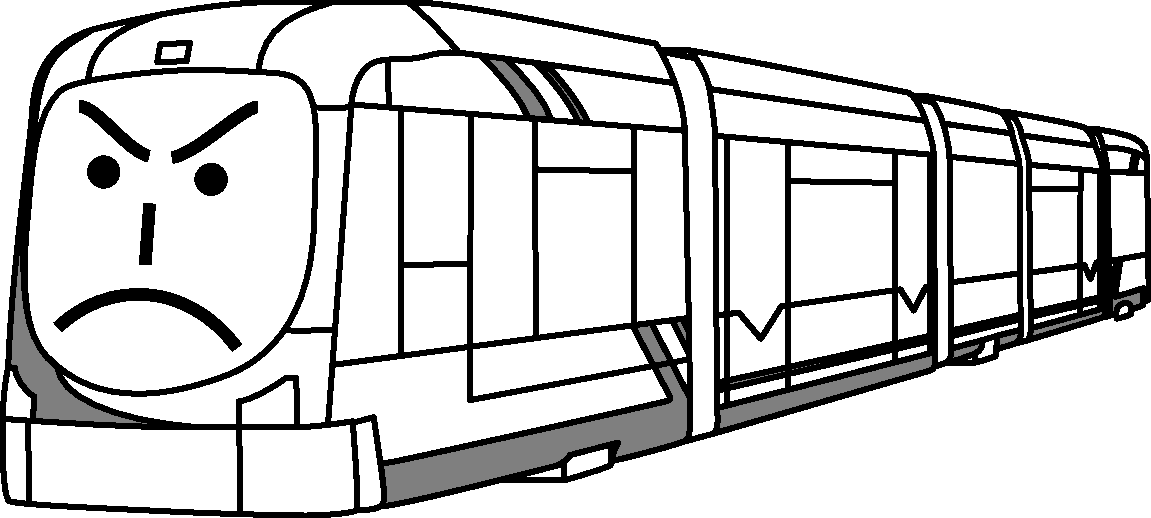
\includegraphics[width=3cm]{bilder/straba.pdf}
}
Seit Herbst 2008 verhandeln die \gls{FSK} und das Studentenwerk mit dem VRN über einen neuen Vertrag. Die \gls{FSK} als studentische Vertretung bei den Verhandlungen fordert ein Ende der enormen Preissteigerungen, um auch in Zukunft mit dem Semesterticket ein günstiges Nahverkehrsangebot zu gewährleisten. Da der VRN jedoch weiter an Preissteigerungen von ca. 10\% pro Jahr festhalten will, stand und steht das Semesterticket vor dem Aus. Nur ein Einlenken in letzter Minute seitens des VRN hat einen Übergangsvertrag im WS 09/10 möglich gemacht. Massiver Druck seitens der Medien, des Rektorats und der Stadt Heidelberg hat dazu geführt, dass die bereits beendeten Verhandlungen wieder aufgenommen worden sind. Bis Ende Oktober müssen sich die Verhandlungsparteien auf einen neuen Vertrag einigen, andernfalls ist das Semesterticket tot.

Die \gls{FSK} und das Studentenwerk versuchen für die Studierenden ein bestmögliches Ticket zu erreichen. Dies bedeutet nicht, dass diese einem inakzeptablen Vertrag zustimmen werden, an den die Studierenden die nächsten fünf Jahre gebunden sind. Selbstverständlich wird dabei aber der Tatsache Rechnung getragen, dass ein Großteil der Studierenden auf den ÖPNV angewiesen ist.\\[2mm]

Heidelberg ist eine eher kleine übersichtliche Stadt in welcher alle Weg bequem mit dem Fahrrad erledigt werden können -- meist sogar schneller als mit Bus und Bahn. Dank der milden Temperaturen ist dies auch im Winter durchaus möglich. Wenn ihr in Heidelberg selbst wohnt ist daher gut zu überlegen ob sich ein Semesterticket lohnt oder man wie viele Andere das Fahrrad nutzt.

Weitere Informationen zu den Verhandlungen und dem Semesterticket findest du unter: \url{http://fachschaftskonferenz.de/semesterticket}

%~ \begin{figure}[h]
%~ \centering{
    %~ 
\includegraphics[width=\textwidth]{bilder/purity.png}
%~ }
%~ \end{figure}


